      
               
                \begin{ledgroupsized}[r]{120mm}
                \footnotesize 
                \pstart                
                \noindent\textbf{\"{U}berlieferung:}   
                \pend
                \end{ledgroupsized}
            
              
                            \begin{ledgroupsized}[r]{114mm}
                            \footnotesize 
                            \pstart \parindent -6mm
                            \makebox[6mm][l]{\textit{L}}Konzept: LH XXXVIII Bl. 172. 1 Bl. 13 x 22 cm. 1 S. Obere und rechte Seite regelm\"{a}ßig, untere Seite unregelm\"{a}ßig beschnitten. R\"{u}ckseite Fragmente algebraischer Rechnungen sowie geometrische Figuren. Die Zeichnung befindet sich am linken Rand. Darunter das Fragment einer abgebrochenen und gestrichenen Rechnung. Eine weitere Rechnung unterhalb des Textes. Beide werden aufgrund der Reihenabgrenzungen hier nicht wiedergegeben.\\Cc 2, Nr. 1188 \pend
                            \end{ledgroupsized}
                %\normalsize
                \vspace*{5mm}
                \begin{ledgroup}
                \footnotesize 
                \pstart
            \noindent\footnotesize{\textbf{Datierungsgr\"{u}nde}: Am linken Seitenrand unten sowie am unteren Seitenrand finden sich Rechnungsfragmente, die große \"{A}hnlichkeit mit den Rechnungen in der Mitte von LH IV, 3, 9 Bl. 10 v\textsuperscript{o} aufweisen. Es ist zu vermuten, dass unsere Fragmente urspr\"{u}nglich mit den erw\"{a}hnten Rechnungen im Zusammenhang standen, die von Leibniz sp\"{a}ter getilgt wurden. Die Rechnungen auf LH IV 3, 9 Bl. 10 v\textsuperscript{o} wurden von Leibniz z. T. \"{u}berschrieben. Der entsprechende Text ist als \textit{LSB} VI 3 N. 71 gedruckt und von Leibniz auf den 15. April 1676 datiert worden. Unser Text muss daher vor diesem Datum entstanden sein. F\"{u}r diese Entstehungszeit spricht zudem sein Wasserzeichen, das sich auch auf den Texttr\"{a}gern von N. 37, N. 74 und N. 75 in \textit{LSB} VI, 3 findet. Die St\"{u}cke sind mit hoher Wahrscheinlichkeit im April 1676 entstanden. Wir nehmen daher f\"{u}r unser St\"{u}ck das Fr\"{u}hjahr 1676 als Entstehungszeitraum an.}
                \pend
                \end{ledgroup}
            
                \vspace*{8mm}
                \pstart 
                \normalsize
            [172 r\textsuperscript{o}] \selectlanguage{french}\textso{Trouuer les }\textso{Pignons}\protect\index{Sachverzeichnis}{pignon}: Supposez que j'aye un pignon\protect\index{Sachverzeichnis}{pignon} divis\'{e} en un  certain nombre de dens, par exemple 6. dont la distance (corde de l'arc)  est le rayon du pignon\protect\index{Sachverzeichnis}{pignon}, on demande un autre pignon\protect\index{Sachverzeichnis}{pignon}, d'un nombre  de dens donn\'{e} par exemple \edtext{18. qui se}{\lemma{18.}\Afootnote{ \textit{ (1) }\ dans les \textit{ (2) }\ le \textit{ (3) }\ qui se \textit{ L}}} puisse mettre  \`{a} la place du premier pignon\protect\index{Sachverzeichnis}{pignon} c'est \`{a} dire dans lequel l'ouuerture  ou distance des dens soit la même, que dans le premier pignon\protect\index{Sachverzeichnis}{pignon},  c'est \`{a} dire soit un cercle \textit{A} divis\'{e} en un certain nombre de parties,  comme 6. La corde d'une sixieme de la \edtext{circomference}{\lemma{circomference}\Afootnote{ \textit{ (1) }\ \textit{AB} \textit{ (2) }\ \textit{CD} \textit{ L}}} \textit{CD} par exemple 4 lignes. \edtext{On demande}{\lemma{lignes.}\Afootnote{ \textit{ (1) }\ Soit \textit{ (2) }\ On demande \textit{ L}}} un autre cercle \textit{B} divis\'{e} en \edtext{18 parties,}{\lemma{18 parties,}\Bfootnote{Leibniz ist zunächst von einer Unterteilung in 14 Abschnitte ausgegangen. Diese Unterteilung hat sich in \textit{[Fig. 1]} erhalten.}} en sorte que la corde d'une 18\textsuperscript{me} partie de sa circomference, comme \textit{EF}, soit egale \`{a} \textit{CD}, corde  de la 6\textsuperscript{me} partie du cercle donn\'{e} \textit{A}. Pour trouuer le cercle \textit{B}, il  suffit de trouuer son rayon \textit{BE}. Cela se fera ainsi. La rayon d'un cercle  estant \edtext{pos\'{e}}{\lemma{estant}\Afootnote{ \textit{ (1) }\ donn\'{e} \textit{ (2) }\ pos\'{e} \textit{ L}}} 100,000, on peut trouuer la corde \edtext{de la 18\textsuperscript{me} de la circomference}{\lemma{corde}\Afootnote{ \textit{ (1) }\ de 18 degrez \textit{ (2) }\ de [...] circomference \textit{ L}}}  par la table de sinus, \edtext{car}{\lemma{sinus,}\Afootnote{ \textit{ (1) }\ o\`{u} le sinus de \textit{ (2) }\ car \textit{ L}}} la 18\textsuperscript{me} partie de la circomference fait 20 degrez, et la corde de 20 degrez est le double du sinus de 10 degrez.  Le sinus de dix degrez est connu par les tables, dont \edtext{son double}{\lemma{dont}\Afootnote{ \textit{ (1) }\ sa corde \textit{ (2) }\ son double \textit{ L}}} aussi, ainsi  la raison du rayon \`{a} cette corde est conn\"{u}e, comme 100,000 est, \`{a} \textit{b}.  Appellons cette raison comme \textit{a} \`{a} \textit{b} donc il est manifeste, que nous aurons cette analogie, ou regle de trois;  comme \textit{b} est \`{a} \textit{a}, ainsi la grandeur conn\"{u}e, \textit{EF}, par exemple 4 lignes,  est \`{a} l'inconnue, ou rayon cherch\'{e}, \textit{BE}, donc \textit{BE}, sera: \begin{tabular}{c|c} 400, & 000 \\ \hline \textit{b} ... & \\ \end{tabular}
            %\includegraphics[width=0.1\textwidth]{images/38_172rcalc1}
            lignes ou \edtext{}{\lemma{}\Afootnote{ou  \textbar\ 400 \textit{ gestr.}\ \textbar\ \textit{ L}}}\selectlanguage{latin}[\textit{Satz bricht ab}]
            \pend
%  Zeitz auskommentiert            \vspace{1.5ex}
%              \begin{center}
%             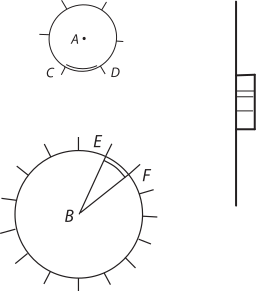
\includegraphics[width=0.4\textwidth]{images/38_172r1}
%              \\\textit{[Fig. 1]}\\
%              \end{center}
%              \protect\index{Sachverzeichnis}{barom\`{e}tre|see{barometrum u. baroscopium}}